% Options for packages loaded elsewhere
\PassOptionsToPackage{unicode}{hyperref}
\PassOptionsToPackage{hyphens}{url}
%
\documentclass[
]{article}
\usepackage{amsmath,amssymb}
\usepackage{iftex}
\ifPDFTeX
  \usepackage[T1]{fontenc}
  \usepackage[utf8]{inputenc}
  \usepackage{textcomp} % provide euro and other symbols
\else % if luatex or xetex
  \usepackage{unicode-math} % this also loads fontspec
  \defaultfontfeatures{Scale=MatchLowercase}
  \defaultfontfeatures[\rmfamily]{Ligatures=TeX,Scale=1}
\fi
\usepackage{lmodern}
\ifPDFTeX\else
  % xetex/luatex font selection
\fi
% Use upquote if available, for straight quotes in verbatim environments
\IfFileExists{upquote.sty}{\usepackage{upquote}}{}
\IfFileExists{microtype.sty}{% use microtype if available
  \usepackage[]{microtype}
  \UseMicrotypeSet[protrusion]{basicmath} % disable protrusion for tt fonts
}{}
\makeatletter
\@ifundefined{KOMAClassName}{% if non-KOMA class
  \IfFileExists{parskip.sty}{%
    \usepackage{parskip}
  }{% else
    \setlength{\parindent}{0pt}
    \setlength{\parskip}{6pt plus 2pt minus 1pt}}
}{% if KOMA class
  \KOMAoptions{parskip=half}}
\makeatother
\usepackage{xcolor}
\usepackage[margin=1in]{geometry}
\usepackage{color}
\usepackage{fancyvrb}
\newcommand{\VerbBar}{|}
\newcommand{\VERB}{\Verb[commandchars=\\\{\}]}
\DefineVerbatimEnvironment{Highlighting}{Verbatim}{commandchars=\\\{\}}
% Add ',fontsize=\small' for more characters per line
\usepackage{framed}
\definecolor{shadecolor}{RGB}{248,248,248}
\newenvironment{Shaded}{\begin{snugshade}}{\end{snugshade}}
\newcommand{\AlertTok}[1]{\textcolor[rgb]{0.94,0.16,0.16}{#1}}
\newcommand{\AnnotationTok}[1]{\textcolor[rgb]{0.56,0.35,0.01}{\textbf{\textit{#1}}}}
\newcommand{\AttributeTok}[1]{\textcolor[rgb]{0.13,0.29,0.53}{#1}}
\newcommand{\BaseNTok}[1]{\textcolor[rgb]{0.00,0.00,0.81}{#1}}
\newcommand{\BuiltInTok}[1]{#1}
\newcommand{\CharTok}[1]{\textcolor[rgb]{0.31,0.60,0.02}{#1}}
\newcommand{\CommentTok}[1]{\textcolor[rgb]{0.56,0.35,0.01}{\textit{#1}}}
\newcommand{\CommentVarTok}[1]{\textcolor[rgb]{0.56,0.35,0.01}{\textbf{\textit{#1}}}}
\newcommand{\ConstantTok}[1]{\textcolor[rgb]{0.56,0.35,0.01}{#1}}
\newcommand{\ControlFlowTok}[1]{\textcolor[rgb]{0.13,0.29,0.53}{\textbf{#1}}}
\newcommand{\DataTypeTok}[1]{\textcolor[rgb]{0.13,0.29,0.53}{#1}}
\newcommand{\DecValTok}[1]{\textcolor[rgb]{0.00,0.00,0.81}{#1}}
\newcommand{\DocumentationTok}[1]{\textcolor[rgb]{0.56,0.35,0.01}{\textbf{\textit{#1}}}}
\newcommand{\ErrorTok}[1]{\textcolor[rgb]{0.64,0.00,0.00}{\textbf{#1}}}
\newcommand{\ExtensionTok}[1]{#1}
\newcommand{\FloatTok}[1]{\textcolor[rgb]{0.00,0.00,0.81}{#1}}
\newcommand{\FunctionTok}[1]{\textcolor[rgb]{0.13,0.29,0.53}{\textbf{#1}}}
\newcommand{\ImportTok}[1]{#1}
\newcommand{\InformationTok}[1]{\textcolor[rgb]{0.56,0.35,0.01}{\textbf{\textit{#1}}}}
\newcommand{\KeywordTok}[1]{\textcolor[rgb]{0.13,0.29,0.53}{\textbf{#1}}}
\newcommand{\NormalTok}[1]{#1}
\newcommand{\OperatorTok}[1]{\textcolor[rgb]{0.81,0.36,0.00}{\textbf{#1}}}
\newcommand{\OtherTok}[1]{\textcolor[rgb]{0.56,0.35,0.01}{#1}}
\newcommand{\PreprocessorTok}[1]{\textcolor[rgb]{0.56,0.35,0.01}{\textit{#1}}}
\newcommand{\RegionMarkerTok}[1]{#1}
\newcommand{\SpecialCharTok}[1]{\textcolor[rgb]{0.81,0.36,0.00}{\textbf{#1}}}
\newcommand{\SpecialStringTok}[1]{\textcolor[rgb]{0.31,0.60,0.02}{#1}}
\newcommand{\StringTok}[1]{\textcolor[rgb]{0.31,0.60,0.02}{#1}}
\newcommand{\VariableTok}[1]{\textcolor[rgb]{0.00,0.00,0.00}{#1}}
\newcommand{\VerbatimStringTok}[1]{\textcolor[rgb]{0.31,0.60,0.02}{#1}}
\newcommand{\WarningTok}[1]{\textcolor[rgb]{0.56,0.35,0.01}{\textbf{\textit{#1}}}}
\usepackage{graphicx}
\makeatletter
\def\maxwidth{\ifdim\Gin@nat@width>\linewidth\linewidth\else\Gin@nat@width\fi}
\def\maxheight{\ifdim\Gin@nat@height>\textheight\textheight\else\Gin@nat@height\fi}
\makeatother
% Scale images if necessary, so that they will not overflow the page
% margins by default, and it is still possible to overwrite the defaults
% using explicit options in \includegraphics[width, height, ...]{}
\setkeys{Gin}{width=\maxwidth,height=\maxheight,keepaspectratio}
% Set default figure placement to htbp
\makeatletter
\def\fps@figure{htbp}
\makeatother
\setlength{\emergencystretch}{3em} % prevent overfull lines
\providecommand{\tightlist}{%
  \setlength{\itemsep}{0pt}\setlength{\parskip}{0pt}}
\setcounter{secnumdepth}{-\maxdimen} % remove section numbering
\ifLuaTeX
  \usepackage{selnolig}  % disable illegal ligatures
\fi
\usepackage{bookmark}
\IfFileExists{xurl.sty}{\usepackage{xurl}}{} % add URL line breaks if available
\urlstyle{same}
\hypersetup{
  pdftitle={Homework\_Basic\_pipeline\_proficiency},
  pdfauthor={Marilyn Harbert},
  hidelinks,
  pdfcreator={LaTeX via pandoc}}

\title{Homework\_Basic\_pipeline\_proficiency}
\author{Marilyn Harbert}
\date{2024-10-21}

\begin{document}
\maketitle

Homework components 1. Load the relevant software libraries 2. Import
the data 3. Use code to count the number of unique articles in the
dataset 4. Remove useless metadata such as ``Los Angeles Times'' and
``ISSN''. See sample code below 5. Tokenize the data, remove stop words,
remove the phrase ``los angeles,'' and create a dataframe of one word
per row 6. Generate a list of the top 20 bigrams 7. Create a ggplot
chart showing the top 20 bigrams 8. Run a sentiment analysis using the
Afinn lexicon 9. At the bottom of the R markdown document, write a 250
word memo describing your key findings. Describe any problems you
encountered in this process.

\begin{Shaded}
\begin{Highlighting}[]
\CommentTok{\# 1. Load the relevant software libraries}

\FunctionTok{library}\NormalTok{(quanteda)}
\end{Highlighting}
\end{Shaded}

\begin{verbatim}
## Warning: package 'quanteda' was built under R version 4.3.3
\end{verbatim}

\begin{verbatim}
## Warning in .recacheSubclasses(def@className, def, env): undefined subclass
## "ndiMatrix" of class "replValueSp"; definition not updated
\end{verbatim}

\begin{verbatim}
## Package version: 4.1.0
## Unicode version: 14.0
## ICU version: 71.1
\end{verbatim}

\begin{verbatim}
## Parallel computing: disabled
\end{verbatim}

\begin{verbatim}
## See https://quanteda.io for tutorials and examples.
\end{verbatim}

\begin{Shaded}
\begin{Highlighting}[]
\FunctionTok{library}\NormalTok{(tidyverse)}
\end{Highlighting}
\end{Shaded}

\begin{verbatim}
## -- Attaching core tidyverse packages ------------------------ tidyverse 2.0.0 --
## v dplyr     1.1.4     v readr     2.1.5
## v forcats   1.0.0     v stringr   1.5.1
## v ggplot2   3.4.4     v tibble    3.2.1
## v lubridate 1.9.3     v tidyr     1.3.1
## v purrr     1.0.2
\end{verbatim}

\begin{verbatim}
## -- Conflicts ------------------------------------------ tidyverse_conflicts() --
## x dplyr::filter() masks stats::filter()
## x dplyr::lag()    masks stats::lag()
## i Use the conflicted package (<http://conflicted.r-lib.org/>) to force all conflicts to become errors
\end{verbatim}

\begin{Shaded}
\begin{Highlighting}[]
\FunctionTok{library}\NormalTok{(tidytext)}
\FunctionTok{library}\NormalTok{(rio)}
\end{Highlighting}
\end{Shaded}

\begin{verbatim}
## Warning: package 'rio' was built under R version 4.3.3
\end{verbatim}

\begin{verbatim}
## 
## Attaching package: 'rio'
## 
## The following object is masked from 'package:quanteda':
## 
##     convert
\end{verbatim}

\begin{Shaded}
\begin{Highlighting}[]
\CommentTok{\#2. Import the data}

\NormalTok{RawChinaData }\OtherTok{\textless{}{-}} \FunctionTok{read\_csv}\NormalTok{(}\StringTok{"ChinaFDI{-}LAT\_tidy.csv"}\NormalTok{)}
\end{Highlighting}
\end{Shaded}

\begin{verbatim}
## New names:
## Rows: 1550 Columns: 5
## -- Column specification
## -------------------------------------------------------- Delimiter: "," chr
## (2): headline, text dbl (3): ...1, article_nmbr, linenumber
## i Use `spec()` to retrieve the full column specification for this data. i
## Specify the column types or set `show_col_types = FALSE` to quiet this message.
## * `` -> `...1`
\end{verbatim}

\begin{Shaded}
\begin{Highlighting}[]
\CommentTok{\# 3. Use code to count the number of unique articles in the dataset}

\FunctionTok{n\_distinct}\NormalTok{(RawChinaData}\SpecialCharTok{$}\NormalTok{article\_nmbr) }
\end{Highlighting}
\end{Shaded}

\begin{verbatim}
## [1] 36
\end{verbatim}

\begin{Shaded}
\begin{Highlighting}[]
\CommentTok{\#4. Remove useless metadata such as "Los Angeles Times" and "ISSN". See sample code below}
\NormalTok{ChinaData\_nometa }\OtherTok{\textless{}{-}}\NormalTok{ RawChinaData }\SpecialCharTok{\%\textgreater{}\%}
  \FunctionTok{mutate}\NormalTok{(}\AttributeTok{text =} \FunctionTok{str\_squish}\NormalTok{(text)) }\SpecialCharTok{\%\textgreater{}\%}
  \FunctionTok{mutate}\NormalTok{(}\AttributeTok{text =} \FunctionTok{tolower}\NormalTok{(text)) }\SpecialCharTok{\%\textgreater{}\%}
  \FunctionTok{mutate}\NormalTok{(}\AttributeTok{text =} \FunctionTok{str\_replace}\NormalTok{(text, }\StringTok{"startofarticle"}\NormalTok{, }\StringTok{""}\NormalTok{)) }\SpecialCharTok{\%\textgreater{}\%}
  \FunctionTok{mutate}\NormalTok{(}\AttributeTok{text =} \FunctionTok{gsub}\NormalTok{(}\StringTok{"issn:}\SpecialCharTok{\textbackslash{}\textbackslash{}}\StringTok{s+}\SpecialCharTok{\textbackslash{}\textbackslash{}}\StringTok{S+"}\NormalTok{, }\StringTok{""}\NormalTok{, text)) }\SpecialCharTok{\%\textgreater{}\%}
  \FunctionTok{mutate}\NormalTok{(}\AttributeTok{text =} \FunctionTok{str\_replace\_all}\NormalTok{(text, }\FunctionTok{c}\NormalTok{(}
    \StringTok{"copyright: (copyright (c) 2005 los angeles times)"} \OtherTok{=} \StringTok{""}\NormalTok{,}
    \StringTok{"database: proquest central"} \OtherTok{=} \StringTok{""}\NormalTok{,}
    \StringTok{"language of publication: english"} \OtherTok{=} \StringTok{""}\NormalTok{,}
    \StringTok{"document url:}\SpecialCharTok{\textbackslash{}\textbackslash{}}\StringTok{s+}\SpecialCharTok{\textbackslash{}\textbackslash{}}\StringTok{S+"} \OtherTok{=} \StringTok{""}\NormalTok{,}
    \StringTok{"proquest document id:}\SpecialCharTok{\textbackslash{}\textbackslash{}}\StringTok{s+}\SpecialCharTok{\textbackslash{}\textbackslash{}}\StringTok{S+"} \OtherTok{=} \StringTok{""}\NormalTok{,}
    \StringTok{"publication subject:}\SpecialCharTok{\textbackslash{}\textbackslash{}}\StringTok{s+}\SpecialCharTok{\textbackslash{}\textbackslash{}}\StringTok{S+"} \OtherTok{=} \StringTok{""}\NormalTok{,}
    \StringTok{"publication date:}\SpecialCharTok{\textbackslash{}\textbackslash{}}\StringTok{s+}\SpecialCharTok{\textbackslash{}\textbackslash{}}\StringTok{S+"} \OtherTok{=} \StringTok{""}\NormalTok{,}
    \StringTok{"pages:}\SpecialCharTok{\textbackslash{}\textbackslash{}}\StringTok{s+}\SpecialCharTok{\textbackslash{}\textbackslash{}}\StringTok{S+"} \OtherTok{=} \StringTok{""}
\NormalTok{  ))) }\SpecialCharTok{\%\textgreater{}\%}
  \FunctionTok{mutate}\NormalTok{(}\AttributeTok{text =} \FunctionTok{str\_replace\_all}\NormalTok{(text, }\FunctionTok{c}\NormalTok{(}
    \StringTok{"search.proquest.com"} \OtherTok{=} \StringTok{""}\NormalTok{,}
    \StringTok{"los angeles times"} \OtherTok{=} \StringTok{""}\NormalTok{,}
    \StringTok{"los angeles"} \OtherTok{=} \StringTok{""}\NormalTok{,}
    \StringTok{"calif"} \OtherTok{=} \StringTok{""}\NormalTok{))) }
\end{Highlighting}
\end{Shaded}

\begin{Shaded}
\begin{Highlighting}[]
\CommentTok{\#5. Tokenize the data, remove stop words, remove the phrase "los angeles," and create a dataframe of one word per row}

\CommentTok{\#Tokenize the data}
\NormalTok{chinadata\_tokenized }\OtherTok{\textless{}{-}}\NormalTok{ ChinaData\_nometa }\SpecialCharTok{\%\textgreater{}\%}
  \FunctionTok{unnest\_tokens}\NormalTok{(bigram,text, }\AttributeTok{token=}\StringTok{"ngrams"}\NormalTok{, }\AttributeTok{n=}\DecValTok{2}\NormalTok{)}

\NormalTok{china\_bigrams\_separated }\OtherTok{\textless{}{-}}\NormalTok{ chinadata\_tokenized }\SpecialCharTok{\%\textgreater{}\%}
  \FunctionTok{separate}\NormalTok{(bigram, }\FunctionTok{c}\NormalTok{(}\StringTok{"word1"}\NormalTok{, }\StringTok{"word2"}\NormalTok{), }\AttributeTok{sep =} \StringTok{" "}\NormalTok{)}

\CommentTok{\#remove stop words and }
\FunctionTok{data}\NormalTok{(stop\_words)}
\NormalTok{china\_bigrams\_separated }\OtherTok{\textless{}{-}}\NormalTok{ china\_bigrams\_separated }\SpecialCharTok{\%\textgreater{}\%}
  \FunctionTok{filter}\NormalTok{(}\SpecialCharTok{!}\NormalTok{word1 }\SpecialCharTok{\%in\%}\NormalTok{ stop\_words}\SpecialCharTok{$}\NormalTok{word) }\SpecialCharTok{\%\textgreater{}\%}
  \FunctionTok{filter}\NormalTok{(}\SpecialCharTok{!}\NormalTok{word2 }\SpecialCharTok{\%in\%}\NormalTok{ stop\_words}\SpecialCharTok{$}\NormalTok{word) }\SpecialCharTok{\%\textgreater{}\%}
  \FunctionTok{filter}\NormalTok{(word1  }\SpecialCharTok{!=} \StringTok{"https"}\NormalTok{) }\SpecialCharTok{\%\textgreater{}\%}
  \FunctionTok{filter}\NormalTok{(word2  }\SpecialCharTok{!=} \StringTok{"https"}\NormalTok{) }\SpecialCharTok{\%\textgreater{}\%}
  \FunctionTok{filter}\NormalTok{(}\SpecialCharTok{!}\FunctionTok{grepl}\NormalTok{(}\StringTok{\textquotesingle{}[0{-}9]\textquotesingle{}}\NormalTok{, word2)) }\SpecialCharTok{\%\textgreater{}\%}
  \FunctionTok{filter}\NormalTok{(}\SpecialCharTok{!}\FunctionTok{grepl}\NormalTok{(}\StringTok{\textquotesingle{}[0{-}9]\textquotesingle{}}\NormalTok{,word2))}

\CommentTok{\#create a dataframe of one word per row}

\NormalTok{chinadata\_tokenized\_fortibble }\OtherTok{\textless{}{-}}\NormalTok{ ChinaData\_nometa }\SpecialCharTok{\%\textgreater{}\%}
  \FunctionTok{unnest\_tokens}\NormalTok{(word,text)}

\NormalTok{chinadata\_tokenized\_fortibble }\OtherTok{\textless{}{-}} \FunctionTok{str\_replace\_all}\NormalTok{(chinadata\_tokenized\_fortibble}\SpecialCharTok{$}\NormalTok{word, }\StringTok{"{-} "}\NormalTok{, }\StringTok{""}\NormalTok{)}
\NormalTok{chinadata\_tokenized\_fortibble }\OtherTok{\textless{}{-}} \FunctionTok{tibble}\NormalTok{(chinadata\_tokenized\_fortibble,)}
\end{Highlighting}
\end{Shaded}

\begin{Shaded}
\begin{Highlighting}[]
\CommentTok{\# 6. Generate a list of the top 20 bigrams}

\NormalTok{count\_china\_bigrams }\OtherTok{\textless{}{-}}\NormalTok{ china\_bigrams\_separated }\SpecialCharTok{\%\textgreater{}\%}
  \FunctionTok{count}\NormalTok{(word1, word2, }\AttributeTok{sort =} \ConstantTok{TRUE}\NormalTok{) }\SpecialCharTok{\%\textgreater{}\%} 
  \FunctionTok{filter}\NormalTok{(}\SpecialCharTok{!}\FunctionTok{is.na}\NormalTok{(word1))}

\NormalTok{top\_20\_bigrams\_china }\OtherTok{\textless{}{-}} \FunctionTok{head}\NormalTok{(count\_china\_bigrams, }\DecValTok{20}\NormalTok{)}
\end{Highlighting}
\end{Shaded}

\begin{Shaded}
\begin{Highlighting}[]
\CommentTok{\#7. Create a ggplot chart showing the top 20 bigrams}
\FunctionTok{library}\NormalTok{(ggplot2)}

\CommentTok{\# join the bigrams into one column for ease}
\NormalTok{top\_20\_bigrams\_china }\OtherTok{\textless{}{-}}\NormalTok{ top\_20\_bigrams\_china }\SpecialCharTok{\%\textgreater{}\%}
  \FunctionTok{unite}\NormalTok{(}\StringTok{"bigram"}\NormalTok{, word1}\SpecialCharTok{:}\NormalTok{word2, }\AttributeTok{remove =} \ConstantTok{FALSE}\NormalTok{)}

\NormalTok{top\_20\_plot }\OtherTok{\textless{}{-}} \FunctionTok{ggplot}\NormalTok{(}
\NormalTok{  top\_20\_bigrams\_china,}
  \FunctionTok{aes}\NormalTok{(}\AttributeTok{x =} \FunctionTok{reorder}\NormalTok{(bigram,n), }\AttributeTok{y =}\NormalTok{ n, }\AttributeTok{fill =}\NormalTok{ n)) }\SpecialCharTok{+}
  \FunctionTok{geom\_col}\NormalTok{(}\AttributeTok{position =} \StringTok{"dodge"}\NormalTok{) }\SpecialCharTok{+} 
  \FunctionTok{theme}\NormalTok{(}\AttributeTok{legend.position =} \StringTok{"none"}\NormalTok{) }\SpecialCharTok{+}
  \FunctionTok{labs}\NormalTok{(}\AttributeTok{title =} \StringTok{"Top 20 bigrams in Los Angeles Times articles about Chinese businesses in the US"}\NormalTok{,}
       \AttributeTok{subtitle =} \StringTok{" "}\NormalTok{,}
       \AttributeTok{caption =} \StringTok{"Graphic by Marilyn Harbert. 2024{-}10{-}21"}\NormalTok{,}
       \AttributeTok{y=}\StringTok{"n"}\NormalTok{,}
       \AttributeTok{x=}\StringTok{"bigram"}\NormalTok{) }\SpecialCharTok{+} 
  \FunctionTok{theme}\NormalTok{(}\AttributeTok{axis.text.x =} \FunctionTok{element\_text}\NormalTok{(}\AttributeTok{angle =} \DecValTok{45}\NormalTok{, }\AttributeTok{vjust =} \DecValTok{1}\NormalTok{, }\AttributeTok{hjust=}\DecValTok{1}\NormalTok{))}

\NormalTok{top\_20\_plot}
\end{Highlighting}
\end{Shaded}

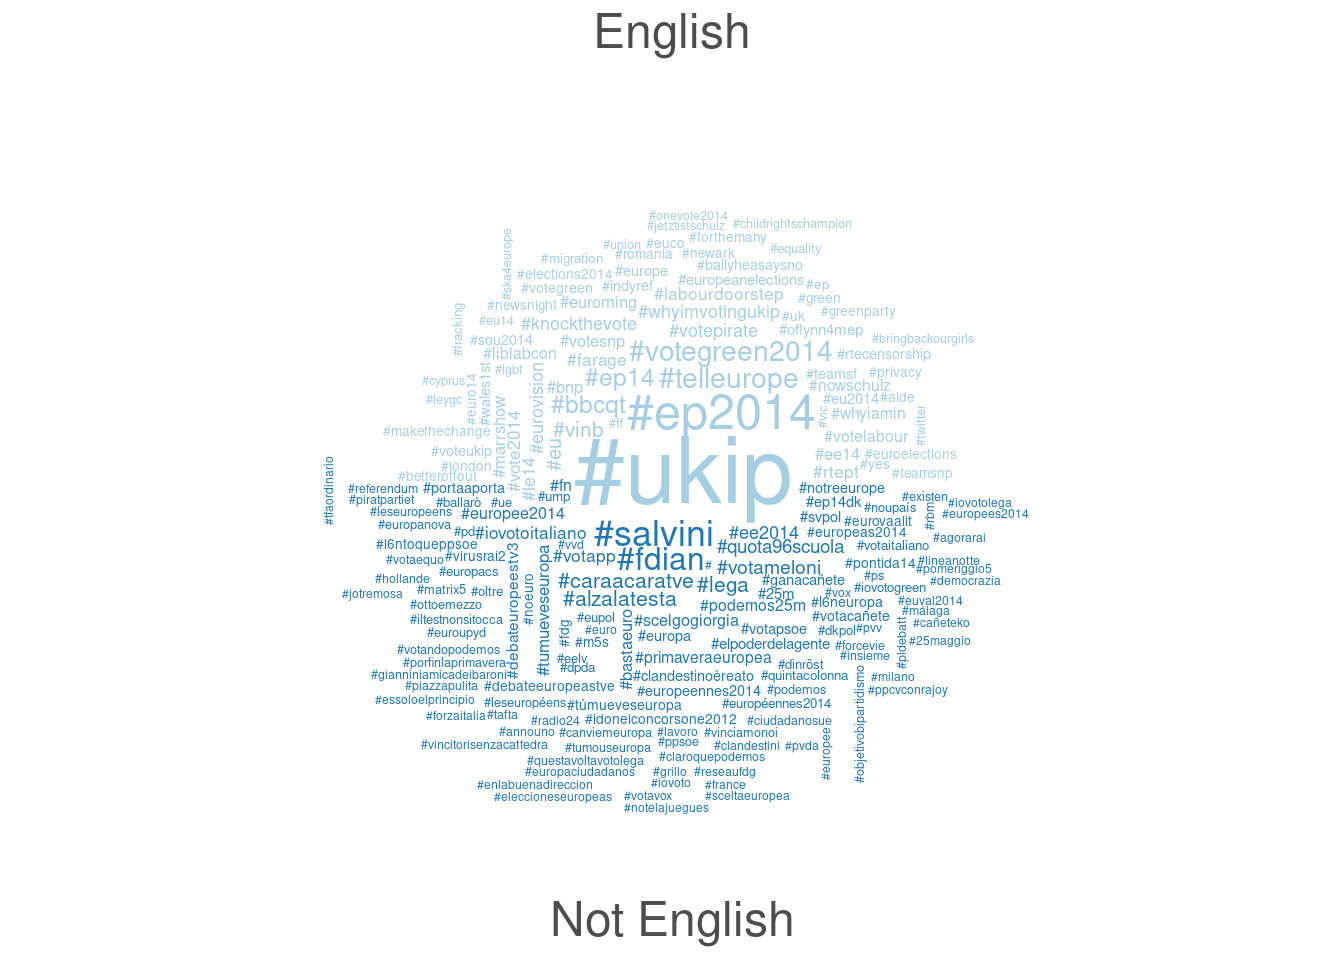
\includegraphics{Homework_Basic_pipeline_proficiency_files/figure-latex/unnamed-chunk-7-1.pdf}

\begin{Shaded}
\begin{Highlighting}[]
\CommentTok{\#8. Run a sentiment analysis using the Afinn lexicon}

\NormalTok{afinn\_sentiments }\OtherTok{\textless{}{-}} \FunctionTok{get\_sentiments}\NormalTok{(}\StringTok{"afinn"}\NormalTok{)}

\NormalTok{sent\_china }\OtherTok{\textless{}{-}}\NormalTok{ china\_bigrams\_separated }\SpecialCharTok{\%\textgreater{}\%}
  \FunctionTok{unite}\NormalTok{(}\StringTok{"bigram"}\NormalTok{, word1}\SpecialCharTok{:}\NormalTok{word2, }\AttributeTok{remove =} \ConstantTok{FALSE}\NormalTok{, }\AttributeTok{sep =} \StringTok{" "}\NormalTok{) }\SpecialCharTok{\%\textgreater{}\%}
  \FunctionTok{unnest\_tokens}\NormalTok{(word, bigram) }\SpecialCharTok{\%\textgreater{}\%}
  \FunctionTok{filter}\NormalTok{(}\SpecialCharTok{!}\NormalTok{word }\SpecialCharTok{\%in\%}\NormalTok{ stop\_words}\SpecialCharTok{$}\NormalTok{word) }\SpecialCharTok{\%\textgreater{}\%}
  \FunctionTok{inner\_join}\NormalTok{(afinn\_sentiments) }\SpecialCharTok{\%\textgreater{}\%}
  \FunctionTok{select}\NormalTok{(linenumber, word, value) }
\end{Highlighting}
\end{Shaded}

\begin{verbatim}
## Joining with `by = join_by(word)`
\end{verbatim}

\begin{enumerate}
\def\labelenumi{\arabic{enumi}.}
\setcounter{enumi}{8}
\tightlist
\item
  At the bottom of the R markdown document, write a 250 word memo
  describing your key findings. Describe any problems you encountered in
  this process.
\end{enumerate}

In this case, I think the bigram analysis tells us more than the
sentiment analysis. From the top 20 bigrams of LA Times articles about
Chinese businesses in the US we can see by the presence of ``Chinese
government'' and ``US government'' that these stories are not just being
framed in terms of Chinese businesses in the US, but that the stories
look at the roles of both governments in this case. The national
security bigram highlights the national security conversation ongoing
around the role of Chinese investment in the US. And the several
``chinese investment'' bigrams show that narratives don't just seem
concerned with Chinese owned businesses, but also where money from
Chinese investment is going.

I found this process harder than I thought it would be! Taking out stop
words and meta data felt like a constant upward battle that I still
probably didn't fully win. And everytime I wanted to do something new to
the data, making sure it was in the form I needed for the new action
took a lot of consideration.

\end{document}
